\chapter{Planar Graphs and Planarity Testing}

Some graphs can be drawn on a sheet of paper without any two edges crossing, and
some cannot. That single distinction -- can it be flattened or not -- turns out to
control an astonishing amount of structure. Planar graphs are sparse ($m\le 3n-6$),
they have small balanced separators, they can be four-colored, and dozens of problems
that are NP-hard in general become polynomial or even linear when the input is
planar. The whole edifice rests on one identity Euler wrote down in 1750 for convex
polyhedra: $V-E+F=2$. We will mine that identity for everything it is worth, prove
that exactly two graphs ($K_5$ and $K_{3,3}$) are the hidden obstructions to
planarity, sketch how a single DFS can test planarity in linear time, and close with
the coloring and separator theorems that make planar graphs the friendliest large
graphs in the business.

\begin{historybox}
The story of planar graphs began in polyhedral geometry. In 1750, Leonhard Euler wrote a
letter to Christian Goldbach stating his famous polyhedral formula: for any convex
polyhedron, $V - E + F = 2$. Euler confirmed it by tabulating vertices, edges, and faces
for prisms, pyramids, and the Platonic solids, but he lacked the topological machinery to
provide a complete proof (formal topology did not exist).

In 1813, Augustin-Louis Cauchy published a celebrated proof: project the polyhedron onto
a plane, excise one face, and triangulate the resulting planar network by removing triangles
one by one. But Cauchy's argument contained a hidden false start: it assumed that every
polyhedron's face boundary is a simple disc and that removing faces never disconnects the
interior. In 1812 and the decades following, Simon Lhuilier and others discovered counterexamples:
polyhedra with tunnels (such as a hollow square picture frame) satisfy $V - E + F = 0$,
proving that Euler's formula is fundamentally a topological invariant governed by the
\emph{genus} of the surface! This controversy formed the centerpiece of Imre Lakatos's
classic work \emph{Proofs and Refutations}.

In algorithmic graph theory, the problem of testing whether an abstract graph can be embedded
in the plane without edge crossings resisted computer science pioneers throughout the 1960s.
Kazimierz Kuratowski (1930) and Klaus Wagner (1937) had characterized planarity by the
absence of $K_5$ and $K_{3,3}$ minors, but searching for Kuratowski subdivisions required
prohibitive $\Oh(n^6)$ time. The breakthrough arrived in 1974, when John Hopcroft and
Robert Tarjan designed the first $\Oh(n)$ linear-time planarity testing algorithm using a
brilliant depth-first search palm-tree decomposition and path embedding, a feat that helped
earn them the 1986 ACM Turing Award.
\end{historybox}

\chapterline

\section{Drawings, embeddings, and faces}
\label{ch26:setup}

Throughout, $\Gph=(V,E)$ is a finite undirected graph with $n=\abs{V}$ and $m=\abs{E}$.
We forbid loops and, for most of the chapter, multiple edges -- they never help a graph
become planar and only clutter the counting.

\begin{definition}[Planar drawing]
\label{ch26:def-drawing}
A \emph{drawing} of $\Gph$ in the plane $\R^2$ maps each vertex to a distinct point and
each edge $\{u,v\}$ to a simple (non-self-intersecting) curve joining the images of $u$
and $v$, such that the curve meets no other vertex and any two curves meet only at
shared endpoints. A graph is \emph{planar} if it admits such a drawing; a fixed drawing
is a \emph{plane graph}, or a \emph{planar embedding}.
\end{definition}

\begin{intuitionbox}
``Planar'' is a property of the abstract graph: \emph{can it be drawn flatly?} A
``plane graph'' is one specific flat drawing. The same planar graph has many essentially
different embeddings, just as a cube can be unfolded many ways. The crossings you see in
a careless drawing are an artifact of \emph{that} drawing, not of the graph. $K_4$ looks
like it must cross if you draw it as a square with both diagonals, but slide one vertex
inside the triangle of the other three and the crossing vanishes.
\end{intuitionbox}

\begin{center}
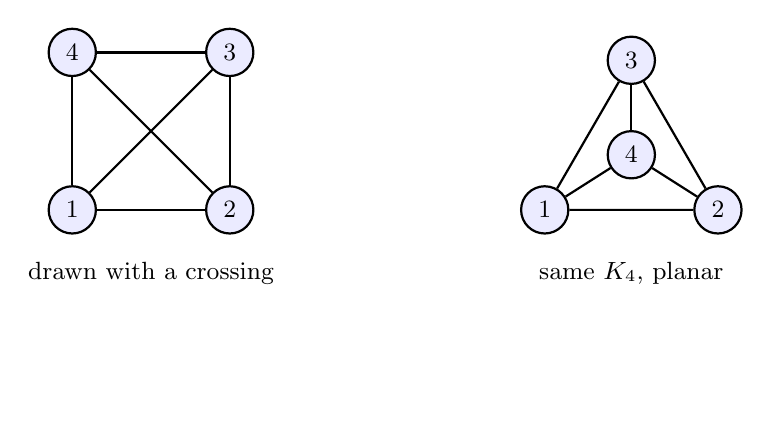
\begin{tikzpicture}[every node/.style={circle,draw,fill=blue!8,minimum size=6mm,inner sep=0pt,font=\small},thick]
  \begin{scope}
    \node (a) at (0,0) {$1$};
    \node (b) at (2,0) {$2$};
    \node (c) at (2,2) {$3$};
    \node (d) at (0,2) {$4$};
    \draw (a)--(b)--(c)--(d)--(a);
    \draw (a)--(c); \draw (b)--(d);
    \node[draw=none,fill=none] at (1,-0.8) {drawn with a crossing};
  \end{scope}
  \begin{scope}[xshift=6cm]
    \node (a) at (0,0) {$1$};
    \node (b) at (2.2,0) {$2$};
    \node (c) at (1.1,1.9) {$3$};
    \node (d) at (1.1,0.7) {$4$};
    \draw (a)--(b)--(c)--(a);
    \draw (a)--(d); \draw (b)--(d); \draw (c)--(d);
    \node[draw=none,fill=none] at (1.1,-0.8) {same $K_4$, planar};
  \end{scope}
\end{tikzpicture}
\end{center}

A plane graph cuts the plane into connected regions called \emph{faces}. One of them is
unbounded -- the \emph{outer} (or infinite) face. The boundary of a face is a closed walk
along edges; an edge can appear on the boundary of one face twice (a bridge), or border
two distinct faces.

\begin{definition}[Face and its degree]
\label{ch26:def-face}
Let $H$ be a plane graph. A \emph{face} is a connected component of $\R^2\setminus H$
(the plane minus all the drawn vertices and edges). The \emph{degree} $\deg(f)$ of a face
$f$ is the number of edges on its boundary walk, counting an edge twice if both of its
sides touch $f$.
\end{definition}

\begin{focusbox}
Three quantities will dance together for the whole chapter: $n$ vertices, $m$ edges, and
$f$ faces of a connected plane graph. Euler's formula ties them so tightly that fixing
any two almost fixes the third.
\end{focusbox}

The two-sided counting of edges around faces is the workhorse identity. Each edge borders
exactly two face-sides (it has a left and a right as you walk along it), so summing face
degrees double-counts edges:
\[
  \sum_{f} \deg(f) \;=\; 2m. \tag{$\star$}
\]
This is the planar cousin of the handshake lemma $\sum_v \deg(v)=2m$, and we will lean on
it constantly.

\section{Euler's formula}
\label{ch26:euler}

\begin{theorem}[Euler's formula]
\label{ch26:thm-euler}
For any connected plane graph with $n$ vertices, $m$ edges, and $f$ faces,
\[
  n - m + f = 2.
\]
\end{theorem}

\begin{intuitionbox}
Grow the graph one edge at a time and watch the bookkeeping. Start from a single vertex:
$n=1$, $m=0$, $f=1$ (just the outer face), and $1-0+1=2$. Now add edges one by one. Every
new edge either reaches a brand-new vertex (a \emph{tree} edge) or closes a cycle (a
\emph{non-tree} edge). A tree edge bumps $n$ and $m$ each by one: $n-m+f$ is unchanged. A
cycle-closing edge splits one face into two, bumping $m$ and $f$ each by one: again
$n-m+f$ is unchanged. The quantity starts at $2$ and never moves.
\end{intuitionbox}

\begin{proof}
Induct on $m$. \emph{Base.} If $m=0$ then $\Gph$ is a single vertex (connected), so
$n=1$, $f=1$, and $1-0+1=2$.

\emph{Step.} Take a connected plane graph with $m\ge 1$ edges and pick any edge $e$.

\emph{Case 1: $e$ lies on a cycle.} Then $e$ borders two distinct faces (its two sides are
in different regions, since the rest of the cycle separates them by the Jordan curve
theorem). Deleting $e$ merges those two faces into one and keeps the graph connected. The
new graph has $n$ vertices, $m-1$ edges, $f-1$ faces; by induction $n-(m-1)+(f-1)=2$,
hence $n-m+f=2$.

\emph{Case 2: $e$ lies on no cycle (a bridge).} Then $e$ has the same face on both sides,
so deleting it does not change $f$, but it disconnects $\Gph$ into two components with
$n_1+n_2=n$, $m_1+m_2=m-1$ edges, and $f_1,f_2$ faces. Each component is a connected plane
graph, but they \emph{share} the outer face, so $f_1+f_2 = f+1$ (the outer face is counted
once in $\Gph$ but once in each piece). Applying induction to each piece,
$n_i-m_i+f_i=2$, and summing,
\[
  n - (m-1) + (f+1) = 4 \;\Longrightarrow\; n-m+f = 2. \qedhere
\]
\end{proof}

\begin{whybox}
The induction is on \emph{a} drawing, but the conclusion $f = 2 - n + m$ shows $f$ does not
depend on which planar drawing you chose -- the number of faces is an invariant of the
abstract planar graph (for connected graphs). That is the first surprising payoff of
Euler: faces feel like a property of the picture, yet their count is forced by $n$ and $m$.
\end{whybox}

\begin{historybox}
Euler announced $V-E+F=2$ for convex polyhedra in 1750 in a letter to Goldbach,
admitting he had no proof. Legendre, Cauchy (1813), and others supplied proofs; Cauchy's
trick of removing a face and flattening the rest into the plane is exactly the
``plane graph'' viewpoint we use. Lakatos's book \emph{Proofs and Refutations} is one long
meditation on the parade of buggy lemmas and patched counterexamples this innocent formula
provoked -- a cautionary tale about ``obvious'' planarity claims.
\end{historybox}

\subsection{The sparsity bounds}

Euler's formula is a tool; the sparsity bounds are what you actually carry around.

\begin{theorem}[Edge bound for simple planar graphs]
\label{ch26:thm-edgebound}
If $\Gph$ is simple, planar, and connected with $n\ge 3$, then
\[
  m \le 3n - 6.
\]
If in addition $\Gph$ is bipartite (girth $\ge 4$), then $m\le 2n-4$.
\end{theorem}

\begin{proof}
Fix a plane embedding with $f$ faces. Because $\Gph$ is simple and $n\ge 3$, every face is
bounded by at least three edges, so $\deg(f)\ge 3$ for every face $f$. Summing and using
$(\star)$,
\[
  2m \;=\; \sum_f \deg(f) \;\ge\; 3f \quad\Longrightarrow\quad f \le \tfrac{2}{3}m.
\]
Plug into Euler's formula $f = 2 - n + m$:
\[
  2 - n + m \le \tfrac{2}{3}m \;\Longrightarrow\; m \le 3n - 6.
\]
If $\Gph$ is bipartite it has no odd cycles, so no triangular faces; every face has
$\deg(f)\ge 4$, giving $2m\ge 4f$, $f\le m/2$, and $2-n+m\le m/2$, i.e.\ $m\le 2n-4$.
\end{proof}

\begin{corollary}[Two non-planar graphs]
\label{ch26:cor-k5k33}
$K_5$ and $K_{3,3}$ are not planar.
\end{corollary}

\begin{proof}
$K_5$ has $n=5$, $m=10$. The bound $3n-6 = 9 < 10$ is violated, so $K_5$ cannot be planar.
$K_{3,3}$ is bipartite with $n=6$, $m=9$. The bipartite bound $2n-4 = 8 < 9$ is violated,
so $K_{3,3}$ is not planar.
\end{proof}

\begin{center}
\begin{tikzpicture}[every node/.style={circle,draw,fill=trapred!18,minimum size=6mm,inner sep=0pt,font=\small},thick,scale=0.95]
  \begin{scope}
    \foreach \i in {0,...,4} {
      \node (k\i) at ({90+72*\i}:1.3) {};
    }
    \foreach \i in {0,...,4} \foreach \j in {0,...,4} {
      \ifnum\i<\j \draw (k\i)--(k\j); \fi
    }
    \node[draw=none,fill=none] at (0,-1.9) {$K_5$: $m=10>9$};
  \end{scope}
  \begin{scope}[xshift=6cm]
    \node (a1) at (0,2) {}; \node (a2) at (1.5,2) {}; \node (a3) at (3,2) {};
    \node (b1) at (0,0) {}; \node (b2) at (1.5,0) {}; \node (b3) at (3,0) {};
    \foreach \a in {a1,a2,a3} \foreach \b in {b1,b2,b3} \draw (\a)--(\b);
    \node[draw=none,fill=none] at (1.5,-0.8) {$K_{3,3}$: $m=9>8$};
  \end{scope}
\end{tikzpicture}
\end{center}

\begin{trapbox}
The bound $m\le 3n-6$ is necessary, not sufficient. A graph can satisfy it and still be
non-planar -- glue a disjoint $K_5$ to a long path and the average gets diluted below the
threshold while the $K_5$ keeps it non-planar. Sparsity rules graphs \emph{out}; it never
rules them \emph{in}. Worse: the bound is for \emph{simple} graphs with $n\ge 3$. For
$n=1,2$ it fails ($n=2$, $m=1$ gives $3n-6=0$). And it assumes connectivity for the clean
Euler count; for a graph with $c$ components the formula is $n-m+f = 1+c$.
\end{trapbox}

\begin{corollary}[A low-degree vertex always exists]
\label{ch26:cor-degree5}
Every simple planar graph has a vertex of degree at most $5$.
\end{corollary}

\begin{proof}
If every vertex had degree $\ge 6$, then $2m=\sum_v\deg(v)\ge 6n$, so $m\ge 3n>3n-6$,
contradicting Theorem~\ref{ch26:thm-edgebound}. (For $n<3$ the claim is trivial.)
\end{proof}

This innocuous corollary is the seed of both the five-color theorem and linear-time planar
algorithms: planar graphs always have a cheap vertex to peel off, so greedy/recursive
strategies terminate fast.

\begin{labbox}
Trace the edge-growing proof on the cube graph $Q_3$ ($n=8$, $m=12$). Euler predicts
$f = 2 - 8 + 12 = 6$ faces -- the six faces of an actual cube, plus you reinterpret one as
the outer face when you flatten it. Now check the bound: $3n-6 = 18 \ge 12$, consistent.
Check $(\star)$: each of the $6$ faces is a $4$-cycle, so $\sum_f\deg(f) = 6\cdot 4 = 24 = 2m$.
Everything closes.
\end{labbox}

\section{Duality}
\label{ch26:duality}

Every face in a planar embedding behaves as a geometric region that can itself be treated as a vertex, giving rise to the dual graph.

\begin{definition}[Dual graph]
\label{ch26:def-dual}
Let $H$ be a connected plane graph. Its \emph{dual} $H^\ast$ has one vertex per face of
$H$, and for each edge $e$ of $H$ a dual edge $e^\ast$ joining the two faces that $e$
borders (a loop if $e$ borders the same face on both sides).
\end{definition}

\begin{figure}[H]
\centering
\begin{tikzpicture}[>=Stealth, scale=1.1]
  \tikzstyle{pv}=[circle,draw=sourceblue,fill=sourceblue!15,thick,minimum size=6.5mm,inner sep=0pt,font=\small\bfseries]
  \tikzstyle{dv}=[circle,draw=quotientorange,fill=quotientorange!20,thick,minimum size=6.5mm,inner sep=0pt,font=\small\bfseries]

  % Primal vertices
  \node[pv] (a) at (0,0)   {$a$};
  \node[pv] (b) at (3.2,0) {$b$};
  \node[pv] (c) at (3.2,2.8) {$c$};
  \node[pv] (d) at (0,2.8) {$d$};
  \node[pv] (e) at (1.6,1.4) {$e$};

  % Primal edges (solid blue)
  \draw[very thick,sourceblue] (a)--(b);
  \draw[very thick,sourceblue] (b)--(c);
  \draw[very thick,sourceblue] (c)--(d);
  \draw[very thick,sourceblue] (d)--(a);
  \draw[very thick,sourceblue] (a)--(e);
  \draw[very thick,sourceblue] (b)--(e);
  \draw[very thick,sourceblue] (c)--(e);
  \draw[very thick,sourceblue] (d)--(e);

  % Dual vertices (inside faces)
  \node[dv] (f1) at (1.6,0.5) {$f_1^\ast$};
  \node[dv] (f2) at (2.5,1.4) {$f_2^\ast$};
  \node[dv] (f3) at (1.6,2.3) {$f_3^\ast$};
  \node[dv] (f4) at (0.7,1.4) {$f_4^\ast$};
  \node[dv] (f0) at (4.6,1.4) {$f_0^\ast$}; % Unbounded outer face

  % Dual edges (dashed orange crossing primal edges orthogonally)
  \draw[thick,dashed,quotientorange] (f1) -- (f2);
  \draw[thick,dashed,quotientorange] (f2) -- (f3);
  \draw[thick,dashed,quotientorange] (f3) -- (f4);
  \draw[thick,dashed,quotientorange] (f4) -- (f1);

  % Connections to exterior face f0*
  \draw[thick,dashed,quotientorange] (f1) to[bend right=25] (f0);
  \draw[thick,dashed,quotientorange] (f2) -- (f0);
  \draw[thick,dashed,quotientorange] (f3) to[bend left=25] (f0);
  \draw[thick,dashed,quotientorange] (f4) to[out=135,in=90,looseness=1.5] (f0);

  % Legend
  \node[font=\footnotesize,sourceblue,anchor=west] at (-0.5,-0.9) {Solid blue: Primal plane graph $H$ ($n=5, m=8, f=5$)};
  \node[font=\footnotesize,quotientorange,anchor=west] at (-0.5,-1.35) {Dashed orange: Orthogonal dual graph $H^\ast$ ($n^\ast=5, m^\ast=8, f^\ast=5$)};
\end{tikzpicture}
\caption{A planar graph $H$ and its orthogonal dual $H^\ast$. Every face of $H$ (four interior triangular faces $f_1, f_2, f_3, f_4$ and one exterior face $f_0$) contains one dual vertex $f^\ast$. Every primal edge $e$ is crossed orthogonally by exactly one dual edge $e^\ast$ connecting the two faces that $e$ borders. Vertices and faces swap roles while the edge count is preserved: $n^\ast = f$, $f^\ast = n$, and $m^\ast = m$.}
\label{ch26:fig-dual-graph}
\end{figure}

Each primal edge crosses exactly its dual edge, so $H$ and $H^\ast$ have the same number of
edges. Vertices and faces swap roles: $n^\ast = f$, $f^\ast = n$, $m^\ast = m$. Euler's
formula is symmetric under this swap -- duality is an involution on connected plane graphs,
$(H^\ast)^\ast = H$.

\begin{connectionbox}
Duality is the bridge to the flow material in Chapters 11--12. In a planar graph, a
\emph{cut} separating $s$ from $t$ corresponds to a \emph{cycle} in the dual separating the
dual faces, and a shortest such cycle is a minimum $s$--$t$ cut. This is how planar min-cut
reduces to planar shortest paths (Reif, Hassin), and why planar max-flow runs much faster
than the general bound. Cuts $\leftrightarrow$ cycles, flows $\leftrightarrow$ potentials --
the same primal/dual duality you met in linear programming, made geometric.
\end{connectionbox}

\begin{remark}
The dual depends on the specific plane embedding rather than the abstract graph alone: a $3$-connected
planar graph has a unique embedding (Whitney's theorem) and hence a unique dual, but
graphs with low connectivity can have several inequivalent embeddings and several duals.
\end{remark}

\section{The forbidden minors: Kuratowski and Wagner}
\label{ch26:kuratowski}

Corollary~\ref{ch26:cor-k5k33} says $K_5$ and $K_{3,3}$ are non-planar. The deep theorem
is the converse: \emph{these are the only obstructions}, provided you look for them in the
right way. Two ways turn out to be equivalent.

\begin{definition}[Subdivision]
A \emph{subdivision} of $\Gph$ replaces some edges by internally disjoint paths (inserting
degree-$2$ vertices along them). Subdividing never affects planarity.
\end{definition}

\begin{definition}[Minor]
A graph $H$ is a \emph{minor} of $\Gph$ if $H$ can be obtained from a subgraph of $\Gph$ by
contracting edges. Equivalently, $H$ is a minor iff $\Gph$ contains $\abs{V(H)}$ disjoint
connected ``branch sets,'' one per vertex of $H$, with an edge of $\Gph$ between branch sets
whenever $H$ has the corresponding edge.
\end{definition}

\begin{theorem}[Kuratowski 1930; Wagner 1937]
\label{ch26:thm-kuratowski}
A graph $\Gph$ is planar if and only if it contains \textbf{no subdivision} of $K_5$ or
$K_{3,3}$ (Kuratowski). Equivalently, $\Gph$ is planar iff it has \textbf{no minor}
isomorphic to $K_5$ or $K_{3,3}$ (Wagner).
\end{theorem}

\begin{intuitionbox}
Both statements say the same thing from two angles. ``Subdivision'' looks for $K_5$ or
$K_{3,3}$ literally drawn out, with the $5$ or $6$ branch vertices and edge-paths between
them threaded through the graph. ``Minor'' is more permissive about how the pieces sit:
each branch vertex can be a whole connected blob you contract to a point. For $K_5$ and
$K_{3,3}$ specifically (all branch degrees $\le 3$ in $K_{3,3}$; degree $4$ in $K_5$), the
two notions coincide, which is why Kuratowski and Wagner are interchangeable here. They
diverge for larger forbidden graphs.
\end{intuitionbox}

\begin{whybox}
\emph{Why necessity is easy, sufficiency is hard.} The ``only if'' direction is just
Corollary~\ref{ch26:cor-k5k33} plus the observation that planarity is closed under taking
subgraphs, subdivisions, and contractions: if $\Gph$ were planar it could not hide a
non-planar $K_5$ or $K_{3,3}$ inside. The ``if'' direction -- that avoiding these two
patterns \emph{guarantees} a flat drawing -- is the content. The cleanest modern proof goes
through $3$-connected graphs: by a theorem of Tutte, every $3$-connected planar graph has a
convex straight-line drawing, and one shows any $3$-connected graph with no $K_5$/$K_{3,3}$
minor is planar by induction on contractions, reducing to $K_4$ as the base. Lower
connectivity is handled by gluing embeddings along cut vertices and separating pairs.
\end{whybox}

We will not reproduce the full $3$-connected case analysis, but the inductive skeleton is
worth seeing because the planarity-testing algorithm mirrors it.

\begin{lemma}[Reduction to $3$-connected pieces]
\label{ch26:lem-3conn}
$\Gph$ is planar iff every one of its blocks (maximal $2$-connected subgraphs, see
Chapter 10) is planar, and a $2$-connected graph is planar iff each of the
$3$-connected components in its SPQR/triconnected decomposition is planar.
\end{lemma}

The point is that planarity is a \emph{local} property of the connectivity skeleton: you may
test it block by block, and within a block, $3$-connected chunk by chunk. Embeddings glue
back together along cut vertices (free choice of which side) and separation pairs (a binary
flip, recorded in the SPQR tree).

\begin{historybox}
Kuratowski proved his theorem in 1930; Wagner's minor version came in 1937. Both are now
seen as the first instance of a vast pattern. Robertson and Seymour's Graph Minor Theorem
(1983--2004) proves that \emph{every} minor-closed family is characterized by a
\emph{finite} list of forbidden minors. Planarity's list happens to have length two. The
catch: Robertson--Seymour is non-constructive about the list for most families, and the
hidden constants are galactic. For planarity we are lucky -- the obstruction set is tiny and
explicit, and testing is linear.
\end{historybox}

\section{Planarity testing}
\label{ch26:testing}

Could we test planarity by hunting for a $K_5$ or $K_{3,3}$ subdivision directly? In
principle yes, but the obvious search is exponential. Three linear-time approaches exist;
all are intricate, so we build intuition for one (the DFS / path-addition family) and
state the guarantees.

\begin{focusbox}
\textbf{Goal.} Decide in $\Oh(n)$ time whether $\Gph$ is planar (and, if so, output an
embedding -- a cyclic edge order at each vertex). Note $m\le 3n-6$ for any candidate, so we
may assume $m=\Oh(n)$: if $m>3n-6$ we instantly answer ``non-planar'' by
Theorem~\ref{ch26:thm-edgebound}. From here on $m=\Oh(n)$, so $\Oh(n)$ and $\Oh(m)$ are the
same.
\end{focusbox}

\subsection{Intuition: add one path at a time}

The path-addition / DFS view (Auslander--Parter, refined by Hopcroft--Tarjan to linear
time) goes like this. Run a DFS, producing a spanning tree plus back edges. Every back edge
closes a cycle with tree edges. Build the embedding incrementally: maintain a partial planar
embedding of what you have placed so far, with a known \emph{outer boundary}, and try to
route each remaining path either inside or outside the current drawing.

The obstruction is a conflict: two pieces that each must be drawn on the same side of an
already-placed cycle, but cannot coexist there. Whether two pieces conflict is captured by a
\emph{$2$-coloring} (inside/outside) of an auxiliary ``interlacement'' graph: pieces that
interlace around the cycle must lie on opposite sides. The graph is planar iff every such
interlacement graph is bipartite; an odd interlacement cycle is exactly a $K_5$ or
$K_{3,3}$ in disguise.

\begin{center}
\begin{tikzpicture}[thick,scale=0.9]
  \tikzstyle{cv}=[circle,draw,fill=blue!10,minimum size=5mm,inner sep=0pt,font=\small]
  \foreach \i/\nm in {0/1,1/2,2/3,3/4,4/5,5/6} {
    \node[cv] (v\i) at ({60*\i}:2) {$\nm$};
  }
  \foreach \i in {0,...,5} {
    \pgfmathtruncatemacro\j{mod(\i+1,6)}
    \draw (v\i)--(v\j);
  }
  \draw[trapred,very thick] (v0) to[bend left=50] (v3);
  \draw[trapred,dashed,very thick] (v1) ..controls (0,-1.2).. (v4);
  \node[draw=none] at (0,-3) {chords $\{1,4\}$ and $\{2,5\}$ \emph{interlace}: their endpoints alternate, so opposite sides are forced};
\end{tikzpicture}
\end{center}

\begin{intuitionbox}
Picture the spanning-tree DFS cycle as a circle. Each remaining piece attaches to the circle
at two or more points. Two pieces \emph{interlace} if their attachment points alternate
around the circle (like $1,2,4,5$ where one piece uses $\{1,4\}$ and the other $\{2,5\}$).
Interlacing pieces cannot both go inside (they would cross) and cannot both go outside, so
one goes in and one goes out. That is a $2$-coloring constraint. A consistent assignment is a
planar embedding; an inconsistency (odd cycle of forced-opposite pieces) is non-planarity.
\end{intuitionbox}

\subsection{A clean recursive scheme}

Here is the Auslander--Parter--Goldstein recursion that makes the idea precise. It is cubic
as written; Hopcroft--Tarjan's bookkeeping squeezes it to linear, but the logic is the same.

\begin{algorithm}[H]
\caption{\textsc{PlanarTest}($\Gph$) -- path-addition skeleton}
\label{ch26:alg-planartest}
\KwIn{a biconnected graph $\Gph$ (test each biconnected block separately).}
\KwOut{\textsc{Planar} or \textsc{NonPlanar}.}
\If{$m > 3n-6$}{\Return \textsc{NonPlanar}\tcp*{sparsity gate, Thm~\ref{ch26:thm-edgebound}}}
\If{$\Gph$ is a single cycle or has $\le 2$ edges}{\Return \textsc{Planar}}
Find a cycle $C$ in $\Gph$\;
Remove $C$; let the connected components of the rest, with their attachments to $C$, be the \emph{bridges} (pieces) $B_1,\dots,B_k$\;
\ForEach{piece $B_i$}{
  recursively embed $B_i \cup (\text{its attachment arcs on } C)$\;
  \lIf{that sub-instance is non-planar}{\Return \textsc{NonPlanar}}
}
Build the \emph{interlacement graph} $I$: a vertex per piece, an edge between pieces whose attachment points interlace around $C$\;
\eIf{$I$ is bipartite}{
  \Return \textsc{Planar}\tcp*{$2$-color = inside/outside assignment}
}{
  \Return \textsc{NonPlanar}\tcp*{odd cycle $\Rightarrow$ $K_5$ or $K_{3,3}$}
}
\end{algorithm}

\begin{whybox}
\emph{Why bipartiteness of the interlacement graph is exactly planarity (around one cycle).}
Each piece must be drawn entirely inside $C$ or entirely outside (a piece is connected and
attaches only on $C$, so it cannot straddle). Interlacing pieces on the same side cross;
non-interlacing pieces on the same side nest peacefully. So a valid drawing is precisely a
$2$-coloring of $I$ with ``same color $\Rightarrow$ non-interlacing,'' i.e.\ a proper
$2$-coloring -- which exists iff $I$ is bipartite. An odd cycle in $I$ is a minimal set of
pieces no side-assignment can satisfy, and unwinding it produces a $K_{3,3}$ or $K_5$
subdivision, recovering Kuratowski. The recursion handles pieces that are themselves complex
by re-running on each piece against its own representative cycle.
\end{whybox}

\begin{complexitybox}
The skeleton recursion is $\Oh(n^3)$ (or $\Oh(n^2)$ with care): $\Oh(n)$ levels, each
building an interlacement graph of size $\Oh(n)$ and bipartiteness-checking it. The
\textbf{Hopcroft--Tarjan} algorithm (1974) reorganizes the same path-additions with a clever
DFS ordering and a stack of conflicts, achieving $\Oh(n)$. The independent
\textbf{vertex-addition} method of Lempel--Even--Cederbaum, sped up by Booth--Lueker's PQ
trees, also runs in $\Oh(n)$. The modern favorite, \textbf{Boyer--Myrvold} (2004), is a
left/right path-addition DFS that is linear, simple to implement, and emits a Kuratowski
subgraph as a certificate of non-planarity.
\end{complexitybox}

\begin{trapbox}
Two classic implementation traps. (1) \emph{Forgetting the sparsity gate.} Without the
$m\le 3n-6$ check, a dense input makes the interlacement graphs huge and the running time
blows up before you even start; always discard $m>3n-6$ first. (2) \emph{Testing
biconnectivity wrong.} Planarity testing is run per biconnected block; if you feed a graph
with a cut vertex straight in, the ``single cycle'' decomposition can miss pieces. Decompose
into blocks (Chapter 10) and test each. A graph is planar iff every block is.
\end{trapbox}

\begin{labbox}
Run the skeleton on $K_4$. Pick the cycle $C = 1\,2\,3\,1$. The remaining vertex $4$ with its
three edges to $1,2,3$ is one piece $B_1$, attaching at $\{1,2,3\}$. There is only one piece,
so the interlacement graph $I$ has a single vertex and no edges, which is immediately bipartite. Answer:
\textsc{Planar}. Now run it on $K_5$. Take $C = 1\,2\,3\,4\,5\,1$. The chords are
$\{1,3\},\{2,4\},\{3,5\},\{4,1\},\{5,2\}$, each its own piece (a single edge). Pieces
$\{1,3\}$ and $\{2,4\}$ interlace; $\{2,4\}$ and $\{3,5\}$ interlace; and so on around a
$5$-cycle of forced-opposite pieces -- an \emph{odd} cycle in $I$. Not bipartite. Answer:
\textsc{NonPlanar}, with the odd $5$-cycle reconstructing the $K_5$ obstruction.
\end{labbox}

\begin{historybox}
Hopcroft and Tarjan's 1974 linear-time planarity test was a landmark -- ``Efficient Planarity
Testing,'' one of the papers that defined what a linear-time graph algorithm should look
like. It is also notoriously hard to implement correctly; for decades the running joke was
that everyone cited it and nobody had coded it. Boyer and Myrvold's 2004 ``On the Cutting Edge''
finally gave a genuinely implementable linear method that also extracts Kuratowski subgraphs,
and it is what most libraries (LEDA, Boost, SageMath) use today.
\end{historybox}

\section{Coloring planar graphs}
\label{ch26:coloring}

The most famous fact about planar graphs is that four colors suffice.

\begin{theorem}[Four Color Theorem; Appel--Haken 1976]
\label{ch26:thm-4ct}
Every planar graph is properly $4$-colorable: its vertices can be colored with four colors so
that adjacent vertices differ.
\end{theorem}

\begin{historybox}
Conjectured by Francis Guthrie in 1852, ``proved'' by Kempe in 1879, and un-proved when
Heawood found the bug in Kempe's argument in 1890 -- though Heawood salvaged enough to get
\emph{five} colors (below). The full theorem fell only in 1976 to Appel and Haken, by a
computer check of $1{,}936$ reducible configurations -- the first major theorem whose proof no
human could verify by hand. Robertson--Sanders--Seymour--Thomas (1997) simplified it to $633$
configurations and a cleaner discharging argument; Gonthier (2005) gave a fully
machine-checked proof in Coq. There is still no ``book proof.''
\end{historybox}

The four-color theorem is hard. The five-color theorem is a beautiful one-page argument that
showcases Corollary~\ref{ch26:cor-degree5} and \emph{Kempe chains}, and it is genuinely
algorithmic.

\begin{theorem}[Five Color Theorem; Heawood 1890]
\label{ch26:thm-5ct}
Every simple planar graph is properly $5$-colorable, and a coloring can be found in
$\Oh(n)$ time.
\end{theorem}

\begin{intuitionbox}
Peel a low-degree vertex, color the rest recursively, then put it back. By
Corollary~\ref{ch26:cor-degree5} there is always a vertex $v$ of degree $\le 5$. If
$\deg(v)\le 4$, its $\le 4$ neighbors use at most $4$ colors and a fifth is free for $v$. The
only hard case is $\deg(v)=5$ with all five colors used by the neighbors. Here we
\emph{recolor} part of the graph to free a color, using a connectivity argument that planarity
makes available -- the Kempe chain.
\end{intuitionbox}

\begin{center}
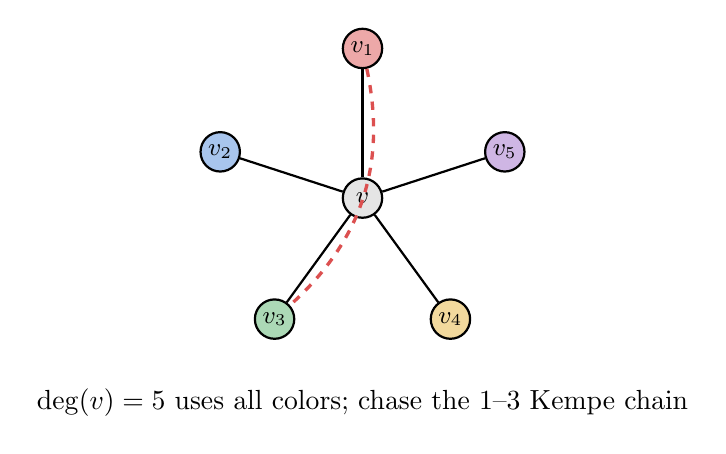
\begin{tikzpicture}[thick,scale=1.0]
  \tikzstyle{n}=[circle,draw,minimum size=5mm,inner sep=0pt,font=\small]
  \definecolor{c1}{RGB}{220,80,80}
  \definecolor{c2}{RGB}{80,140,220}
  \definecolor{c3}{RGB}{90,180,110}
  \definecolor{c4}{RGB}{230,180,60}
  \definecolor{c5}{RGB}{160,110,200}
  \node[n,fill=gray!20] (v) at (0,0) {$v$};
  \node[n,fill=c1!50] (v1) at (90:1.9) {$v_1$};
  \node[n,fill=c2!50] (v2) at (162:1.9) {$v_2$};
  \node[n,fill=c3!50] (v3) at (234:1.9) {$v_3$};
  \node[n,fill=c4!50] (v4) at (306:1.9) {$v_4$};
  \node[n,fill=c5!50] (v5) at (18:1.9) {$v_5$};
  \foreach \i in {1,...,5} \draw (v)--(v\i);
  \draw[c1,very thick,dashed] (v1) to[bend left=30] (v3);
  \node[draw=none] at (0,-2.6) {$\deg(v)=5$ uses all colors; chase the $1$--$3$ Kempe chain};
\end{tikzpicture}
\end{center}

\begin{proof}
Induct on $n$. For $n\le 5$ color arbitrarily. For $n>5$, pick $v$ with $\deg(v)\le 5$
(Corollary~\ref{ch26:cor-degree5}). Delete $v$, $5$-color $\Gph-v$ by induction, and try to
extend.

If $\deg(v)\le 4$, or if $\deg(v)=5$ but the neighbors use $\le 4$ colors, a free color exists;
assign it to $v$. The remaining case: $\deg(v)=5$ and its neighbors $v_1,\dots,v_5$
(in clockwise embedding order) carry all five distinct colors $1,2,3,4,5$.

\emph{Kempe chain.} Look at the subgraph $H_{1,3}$ induced by colors $1$ and $3$. Consider the
connected component of $H_{1,3}$ containing $v_1$ (color $1$).

\emph{Case A: $v_3$ (color $3$) is \emph{not} in that component.} Swap colors $1\leftrightarrow 3$
throughout that component. This keeps a proper coloring (the component's boundary touches only
colors $\ne 1,3$), and now $v_1$ has color $3$. Color $1$ is freed at $v$; assign it.

\emph{Case B: $v_3$ \emph{is} in that component.} Then there is a path $P_{1,3}$ from $v_1$ to
$v_3$ using only colors $1$ and $3$. Together with $v$ this path forms a closed curve. By the
Jordan curve theorem, it separates $v_2$ from $v_4$: one is strictly inside the loop, the other
outside. Now look at $H_{2,4}$, the subgraph on colors $2$ and $4$, and the component
containing $v_2$. Any $2$--$4$ path from $v_2$ to $v_4$ would have to cross $P_{1,3}$ -- but
crossing is impossible in a plane graph and the colors $\{2,4\}$ and $\{1,3\}$ are disjoint, so
no such path exists. Hence $v_2$ and $v_4$ lie in different components of $H_{2,4}$. Swap
$2\leftrightarrow 4$ in $v_2$'s component; color $2$ is freed at $v$. Assign it.
\end{proof}

\begin{whybox}
The Jordan-curve step is where planarity does the heavy lifting. In a non-planar graph the
$1$--$3$ chain need not separate $v_2$ from $v_4$, and the argument collapses -- which is why
$5$ (and $4$) colors are special to the plane. Kempe's 1879 ``proof'' of \emph{four} colors
tried to run two chain swaps at once; Heawood's counterexample showed the two swaps can
interfere. For \emph{five} colors one swap always suffices, and there is no interference.
\end{whybox}

\begin{algorithm}[H]
\caption{\textsc{FiveColor}($\Gph$) -- recursive Kempe-chain coloring}
\label{ch26:alg-fivecolor}
\KwIn{simple planar graph $\Gph$.}
\KwOut{a proper coloring $c:V\to\{1,2,3,4,5\}$.}
\If{$\abs{V}\le 5$}{color all vertices distinctly; \Return}
Find $v$ with $\deg(v)\le 5$\tcp*{exists by Cor.~\ref{ch26:cor-degree5}}
$c \gets \textsc{FiveColor}(\Gph - v)$\;
\eIf{some color in $\{1,\dots,5\}$ is missing among $v$'s neighbors}{
  assign $v$ that color\;
}{
  $v_1,\dots,v_5 \gets$ neighbors in embedding order, with distinct colors\;
  run the Kempe swap on chain $\{c(v_1),c(v_3)\}$ (else $\{c(v_2),c(v_4)\}$) to free a color\;
  assign $v$ the freed color\;
}
\Return $c$\;
\end{algorithm}

\begin{complexitybox}
Each recursion deletes one vertex, so there are $n$ levels. The work per level is finding a
low-degree vertex (amortized $\Oh(1)$ with a degree-bucket queue) and at most one Kempe swap,
which is a BFS/DFS over a $2$-colored subgraph in $\Oh(n)$. Naively $\Oh(n^2)$; with care
about which chains get re-traversed, $\Oh(n)$ total. Four-coloring in polynomial time is also
known (a quadratic algorithm follows from the RSST proof), but it is vastly more involved.
\end{complexitybox}

\begin{trapbox}
A tempting wrong simplification: ``every planar graph is $4$-colorable, so just be greedy and
back off.'' Greedy coloring in a bad vertex order can need up to $\Delta+1$ colors even on a
planar graph -- it does not magically find a $4$- or $5$-coloring. The five-color guarantee
needs the \emph{specific} peel-lowest-degree order \emph{and} the Kempe-chain repair. Drop
either and the bound breaks.
\end{trapbox}

\begin{applicationbox}
Coloring planar graphs is the math behind frequency assignment on a map of transmitters
(adjacent regions need different frequencies), register interference for certain structured
programs, and -- historically -- coloring actual maps, which is the dual statement: countries
become vertices, shared borders become edges, and a map is always planar.
\end{applicationbox}

\section{Planar separators}
\label{ch26:separators}

The last structural gift of planarity is that planar graphs fall apart cleanly: you can always
cut them into balanced halves by deleting only $\Oh(\sqrt n)$ vertices. (The dedicated
separator chapter, Chapter 27, develops this in full; here we state it and read off
consequences.)

\begin{theorem}[Lipton--Tarjan Planar Separator Theorem, 1979]
\label{ch26:thm-separator}
Let $\Gph$ be an $n$-vertex planar graph. There is a partition $V = A \cup S \cup B$ such that
\begin{itemize}
  \item no edge joins $A$ and $B$ (so $S$ \emph{separates} them),
  \item $\abs{A},\abs{B} \le \tfrac{2}{3}n$ (the parts are balanced),
  \item $\abs{S} \le 2\sqrt{2}\,\sqrt n = \Oh(\sqrt n)$ (the separator is small),
\end{itemize}
and $A,S,B$ can be found in $\Oh(n)$ time.
\end{theorem}

\begin{intuitionbox}
Run a BFS from any root. The graph stratifies into levels $L_0,L_1,\dots$ Two facts collide
to give the theorem. First, since $\sum_i \abs{L_i}=n$, \emph{some} level is small -- there is
a level with $\Oh(\sqrt n)$ vertices not too far from the median, and deleting one level
disconnects the levels above from those below. Second, the levels between two such small levels
form a planar graph of bounded ``radius,'' and a bounded-radius planar graph has a small
separator because you can contract the inside to a point and use the fact that a planar graph
with a spanning tree of depth $d$ has a fundamental-cycle separator of size $\Oh(d)$. Balancing
the two effects gives $\Oh(\sqrt n)$. The square root is the perimeter-vs-area scaling of the
plane: a region of $n$ cells has boundary $\sim\sqrt n$.
\end{intuitionbox}

\begin{whybox}
\emph{Why $\sqrt n$ and not less.} The $\sqrt n\times\sqrt n$ grid is planar, and any balanced
separator of it must contain $\Om(\sqrt n)$ vertices -- a horizontal or vertical cut already
costs $\sqrt n$, and one can show no cleverer cut does asymptotically better. So
Lipton--Tarjan is tight up to the constant. Compare: a tree (planar, but a special case) has a
\emph{single-vertex} centroid separator; general graphs (e.g.\ expanders, Chapter 34) need
$\Om(n)$. Planar graphs sit in the sweet spot.
\end{whybox}

\begin{corollary}[Divide and conquer for free]
\label{ch26:cor-sep-divide}
Recursively applying the separator yields a separator hierarchy. This drives:
\begin{itemize}
  \item exact and approximate algorithms running in $2^{\Oh(\sqrt n)}$ for problems that are
        $2^{\Oh(n)}$ in general (planar TSP, planar independent set, planar Hamiltonicity --
        the ``square-root phenomenon'');
  \item nested dissection: solving an $n$-variable planar linear system (e.g.\ a planar
        Laplacian) in $\Oh(n^{3/2})$ time and $\Oh(n\log n)$ fill, by eliminating along the
        separator tree;
  \item polynomial-time approximation schemes via Baker's layering technique.
\end{itemize}
\end{corollary}

\begin{connectionbox}
The separator theorem is the planar gateway to the spectral and Laplacian chapters. Nested
dissection (Corollary~\ref{ch26:cor-sep-divide}) is the fastest classical direct solver for
planar Laplacian systems and feeds straight into the electrical-flow material of Chapter 35.
And the $\Oh(\sqrt n)$ bound is mirrored spectrally: planar graphs have a small second
Laplacian eigenvalue, so Cheeger's inequality (Chapter 32) predicts a sparse cut -- the
separator and the spectral gap are two views of the same flatness.
\end{connectionbox}

\begin{applicationbox}
Planar separators power route planners (road networks are nearly planar; contraction
hierarchies and customizable route planning exploit small separators), VLSI layout (Lipton
and Tarjan's original motivation was circuit area lower bounds), and mesh partitioning for
finite-element solvers, where a good separator is a good way to split work across processors.
\end{applicationbox}

\section{What planarity buys you}
\label{ch26:summary}

\begin{center}
\begin{tabular}{@{}lll@{}}
\toprule
Quantity / problem & General graphs & Planar graphs \\
\midrule
Edges & up to $\binom{n}{2}$ & $\le 3n-6$ \\
Min vertex degree & up to $n-1$ & $\le 5$ \\
Chromatic number & up to $n$ & $\le 4$ \\
Balanced separator & up to $\Om(n)$ & $\Oh(\sqrt n)$ \\
Planarity test & --- & $\Oh(n)$ \\
Max-flow / min-cut & $\Oh(nm)$-ish & near-linear (via duality) \\
Shortest paths (neg.\ ok) & $\Oh(nm)$ & near-linear \\
Independent set, TSP & $2^{\Oh(n)}$ & $2^{\Oh(\sqrt n)}$ \\
\bottomrule
\end{tabular}
\end{center}

The thread tying every row together is Euler's formula. Sparsity ($m\le 3n-6$) comes straight
from it; the low-degree vertex and the colorings come from sparsity; planarity testing
exploits the bounded structure; duality turns cuts into cycles; and separators exploit the
plane's area-perimeter scaling. Learn to see $n-m+f=2$ behind each of them.

\begin{connectionbox}
\textbf{What This Unlocked:}
Planar graphs turn classical computational hardness on its head. Sparsity ($m \le 3n - 6$)
means algorithms that are $\Oh(m)$ run in strict $\Oh(n)$ linear time. Planar duality turns
minimum cuts into shortest cycles in the dual graph, allowing near-linear min-cut and max-flow
computations. Furthermore, planar graphs guarantee vertices of degree at most $5$, enabling
fast recursive reductions and the Four-Color Theorem.

\textbf{Honest Downsides and Limitations:}
\begin{itemize}
  \item \emph{Fragility under minor perturbations:} Planarity is topologically brittle. Adding
        even two or three crossing edges (such as a $K_{3,3}$ subdivision) destroys planarity,
        invalidating Euler's formula and face duality.
  \item \emph{Non-uniqueness of embeddings:} A 2-connected planar graph can have exponentially
        many distinct planar embeddings (differing in face structures), meaning dual-graph algorithms
        must fix an embedding first. Only 3-connected planar graphs enjoy unique embeddings (Whitney 1932).
  \item \emph{Still NP-hard:} Many hard problems remain NP-hard on planar graphs: 3-Coloring,
        Maximum Independent Set, Hamiltonian Cycle, and Vertex Cover remain strictly NP-complete.
\end{itemize}

\textbf{Where We Go Next:}
While planar problems remain NP-hard, their planar geometry enables divide-and-conquer strategies
that run in subexponential time $2^{\Oh(\sqrt{n})}$. In \textbf{Chapter~27 (Separators)}, we
develop the Lipton--Tarjan Planar Separator Theorem, showing that every planar graph can be split
into balanced pieces by deleting only $\Oh(\sqrt{n})$ vertices. And in \textbf{Chapter~28 (Graph
Coloring)}, we explore how planarity ignited the century-long quest for Kempe chains and the
Four-Color Theorem.
\end{connectionbox}

\section{Exercises}
\label{ch26:exercises}

\begin{exercise}[Euler bookkeeping]
A connected planar graph has every face of degree exactly $5$ and every vertex of degree
exactly $3$. Use $(\star)$, the handshake lemma, and Euler's formula to solve for $n$, $m$,
$f$. (You should recognize the dodecahedron.)
\end{exercise}

\begin{exercise}[The component correction]
Prove that for a planar graph with $c$ connected components, $n - m + f = 1 + c$. Where in the
proof of Theorem~\ref{ch26:thm-euler} does connectivity get used, and how does adding a
component change the face count?
\end{exercise}

\begin{exercise}[Girth bound]
Generalize Theorem~\ref{ch26:thm-edgebound}: if a simple planar graph has girth (shortest cycle
length) $g \ge 3$, prove $m \le \frac{g}{g-2}(n-2)$. Recover the $3n-6$ and $2n-4$ bounds as
special cases. Use it to give a one-line proof that the Petersen graph ($n=10$, $m=15$,
girth $5$) is non-planar.
\end{exercise}

\begin{exercise}[Both obstructions are needed]
Exhibit a graph that contains a $K_5$ subdivision but no $K_{3,3}$ subdivision, and another
with a $K_{3,3}$ subdivision but no $K_5$ subdivision. Conclude that neither forbidden graph
alone characterizes planarity.
\end{exercise}

\begin{exercise}[Maximal planar = triangulation]
A planar graph is \emph{maximal planar} if adding any edge destroys planarity. Prove that a
maximal planar graph on $n\ge 3$ vertices has exactly $m = 3n-6$ edges and every face
(including the outer one) is a triangle. (Hint: a non-triangular face has a missing chord you
could add.)
\end{exercise}

\begin{exercise}[Self-dual graphs]
Show that for a self-dual connected plane graph ($H \cong H^\ast$) we have $m = 2n - 2$. Find a
small self-dual example. (Hint: $n = f$ for self-duality; combine with Euler.)
\end{exercise}

\begin{exercise}[Implement five-coloring]
Implement Algorithm~\ref{ch26:alg-fivecolor}. Maintain a bucket queue keyed by current degree so
that finding a $\deg \le 5$ vertex is $\Oh(1)$ amortized, and implement the Kempe swap as a BFS
over the relevant two-color class. Test it on a random maximal planar graph (build one by
repeatedly inserting a vertex into a random triangle) and verify the coloring is proper.
\end{exercise}

\begin{exercise}[Break a naive tester]
Consider the ``tester'' that returns \textsc{Planar} iff $m \le 3n - 6$. Construct an infinite
family of non-planar graphs that this tester wrongly accepts, with $m$ as small as $2n$. Why
does the sparsity gate in Algorithm~\ref{ch26:alg-planartest} not suffer from this -- what does
the rest of the algorithm add?
\end{exercise}

\begin{exercise}[Kempe's mistake]
Read Heawood's counterexample to Kempe's four-color argument. Describe, on a concrete small
configuration, two Kempe chains whose simultaneous swap interferes (one swap undoes the gain of
the other). Explain why a single swap in the five-color proof never has this problem.
\end{exercise}

\begin{exercise}[Separator on the grid]
For the $\sqrt n \times \sqrt n$ grid, prove that any partition $V = A\cup S\cup B$ with
$\abs{A},\abs{B}\ge n/3$ and no $A$--$B$ edge has $\abs{S} = \Om(\sqrt n)$. (Hint: count
rows/columns that must contain a separator vertex.) Conclude that Theorem~\ref{ch26:thm-separator}
is tight up to the constant.
\end{exercise}

\begin{exercise}[Outerplanar warm-up]
A graph is \emph{outerplanar} if it has a planar drawing with every vertex on the outer face.
Prove that an outerplanar simple graph satisfies $m \le 2n - 3$, and that the forbidden minors
for outerplanarity are $K_4$ and $K_{2,3}$. (Reduce to the planar case by adding a new vertex
adjacent to all others and applying Kuratowski.)
\end{exercise}

\begin{exercise}[Dual of a cut]
Let $\Gph$ be a connected plane graph and $H^\ast$ its dual. Prove that a set of edges forms a
minimal edge cut (bond) in $\Gph$ if and only if the corresponding dual edges form a simple
cycle in $H^\ast$. Explain how this lets you compute a minimum $s$--$t$ cut in a planar graph
by a shortest-path computation in the dual.
\end{exercise}
